\section{Results and Discussion}\label{results-and-discussion}

The completed test experiments show a clear accuracy--runtime tradeoff. Sampled-proposal PEARL achieves the strongest point accuracy and reference-plane overlap, sequential RANSAC is fastest, and the hybrid improves the RANSAC segmentation at intermediate cost. Removing spatial regularization causes a large loss of segmentation quality in the selected PEARL configuration. All summaries below use the saved per-case measurements and predictions, with 360 scan--variant--seed records per method; no segmentation was rerun to produce these figures.

\subsection{Three way segmentation comparison}\label{three-way-segmentation-comparison}

Table~\ref{tab:comparison} and Fig.~\ref{fig:results_three_way} compare the three pipelines under the frozen parameter configuration. Sampled PEARL attains 84.26\% mean matched point accuracy, compared with 69.89\% for RANSAC and 77.98\% for the hybrid. Its gain over RANSAC is 14.37 percentage points, or 20.56\% relative to the baseline accuracy. The hybrid gains 8.08 percentage points, or 11.56\% relative. Point-weighted accuracies are nearly identical to the corresponding record means, consistent with the common sampling policy.

The same ordering holds for mean matched IoU and F-score. Sampled PEARL increases mean matched IoU from 0.2086 to 0.4554, a relative improvement of 118.26\%; the hybrid reaches 0.2836, a 35.91\% relative improvement. These plane-weighted scores are substantially lower than point accuracy because recovering a large support does not compensate for missing many smaller reference planes. The aggregate accuracy ordering is unchanged across the three seeds; their method-specific aggregate means span less than 0.5 percentage points. This does not imply that individual cases are insensitive to initialization.

\begin{table*}[!t]
\caption{Three-way comparison on 360 test records per method. Accuracy is mean \(\pm\) descriptive standard deviation; these are correlated records, not independent samples. Mean matched IoU and F-score follow Section~\ref{dataset-and-experimental-setup}. Runtime comes from the initialization-comparison run only.}
\label{tab:comparison}
\centering\footnotesize
\begin{tabular}{lrrrr}
\hline
\shortstack{Method} & \shortstack{Accuracy\\(\%)} & \shortstack{Matched\\IoU} & \shortstack{F-score} & \shortstack{Total\\time\\(s)} \\ \hline
RANSAC & 69.89 \(\pm\) 9.74 & 0.2086 & 0.2257 & 0.376 \\
Sampled PEARL & 84.26 \(\pm\) 8.31 & 0.4554 & 0.4003 & 19.620 \\
Hybrid & 77.98 \(\pm\) 9.47 & 0.2836 & 0.3443 & 2.512 \\
\hline
\end{tabular}
\end{table*}

\begin{figure*}[!t]
\centering
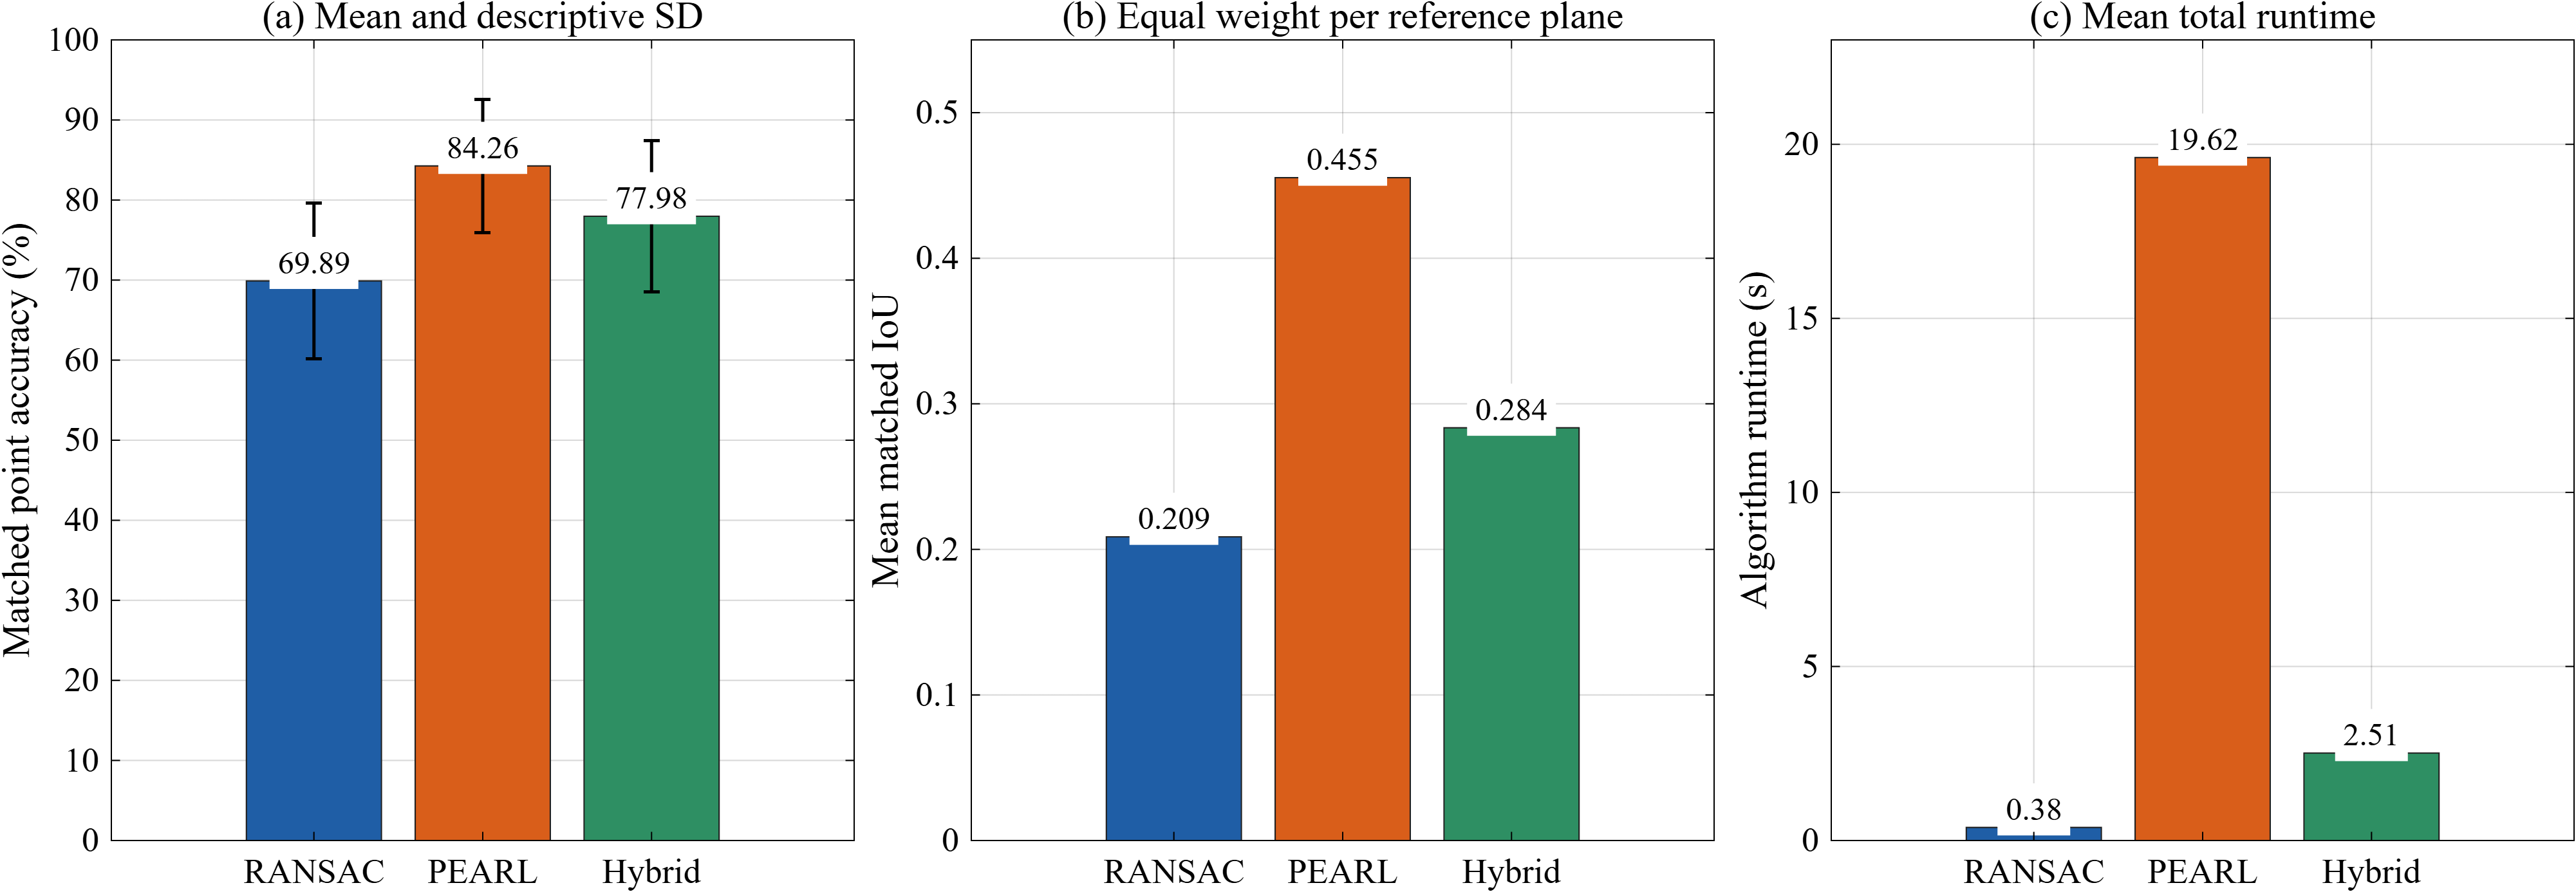
\includegraphics[width=\textwidth]{figures/results_three_way.png}
\caption{Accuracy, reference-plane overlap, and algorithm runtime from the same three-way comparison run. PEARL denotes the sampled-proposal pipeline. Error bars in (a) show descriptive variation across records and are not confidence intervals. The hybrid includes the cost of its RANSAC initialization.}
\label{fig:results_three_way}
\end{figure*}

\subsection{Computational cost and model bank size}\label{computational-cost-and-model-bank-size}

RANSAC requires 0.376 s per record on average, the hybrid 2.512 s, and sampled PEARL 19.620 s. The hybrid is about 7.81 times faster than sampled PEARL, while retaining lower accuracy and overlap; it remains 6.68 times slower than standalone RANSAC. Sampled PEARL costs about 52.20 times the RANSAC runtime in this run. These ratios describe the MATLAB implementations and selected settings, rather than intrinsic complexity constants of the algorithms.

Table~\ref{tab:components} separates initialization from refinement. Sampled PEARL generates its proposal bank in only 0.135 s, whereas RANSAC initialization requires 0.376 s. The hybrid's runtime advantage therefore comes from the subsequent refinement stage rather than a faster initializer. Its mean refinement time is 2.137 s, compared with 19.484 s for sampled PEARL. The smaller model bank is consistent with this difference: the hybrid begins with 19.12 planes on average, while sampled PEARL begins with 150. Each expansion sweep visits every available label, making bank size relevant to graph-cut workload. The experiment does not independently control bank size to establish it as the sole cause.

\begin{table*}[!t]
\caption{Mean model counts and runtime components. ``At cap'' counts records that complete all 15 outer iterations, out of 360. The reference contains 40.93 planes per sampled scan--variant input on average. RANSAC has no PEARL iteration count.}
\label{tab:components}
\centering\footnotesize
\begin{tabular}{lrrrrr}
\hline
\shortstack{Method} & \shortstack{Initial\\planes} & \shortstack{Final\\planes} & \shortstack{Init.\\time\\(s)} & \shortstack{Refine\\time\\(s)} & \shortstack{At\\cap} \\ \hline
RANSAC & 19.12 & 19.12 & 0.376 & 0.000 & --- \\
Sampled PEARL & 150.00 & 54.25 & 0.135 & 19.484 & 89 \\
Hybrid & 19.12 & 19.09 & 0.376 & 2.137 & 60 \\
\hline
\end{tabular}
\end{table*}

The hybrid finishes with 19.09 planes on average and cannot add labels beyond its RANSAC bank. Its mean instance precision is 0.4903, greater than sampled PEARL's 0.3776, but its recall is lower, 0.2743 versus 0.4501. This is consistent with a smaller collection of detected planes that leaves more reference structures unrecovered. Sampled PEARL ends with 54.25 planes on average, showing that unused labels are removed, although this does not guarantee the correct model count. The iteration cap is reached in 89 sampled-PEARL records and 60 hybrid records. Further energy reduction may therefore be possible in some cases, without a guarantee of higher accuracy.

\subsection{Paired refinement and energy reduction}\label{paired-refinement-and-energy-reduction}

Starting from the exact RANSAC output, the hybrid improves point accuracy in 357 of 360 records and reduces it in three; there are no ties at the reporting tolerance. Mean matched IoU increases by 0.0749 and mean F-score by 0.1187. Independently recomputed energy does not increase in any paired case, and its mean decrease is 0.5041 in the original squared-distance units. Fig.~\ref{fig:results_paired_energy} distinguishes this optimization behavior from reference-label accuracy.

\begin{figure*}[!t]
\centering
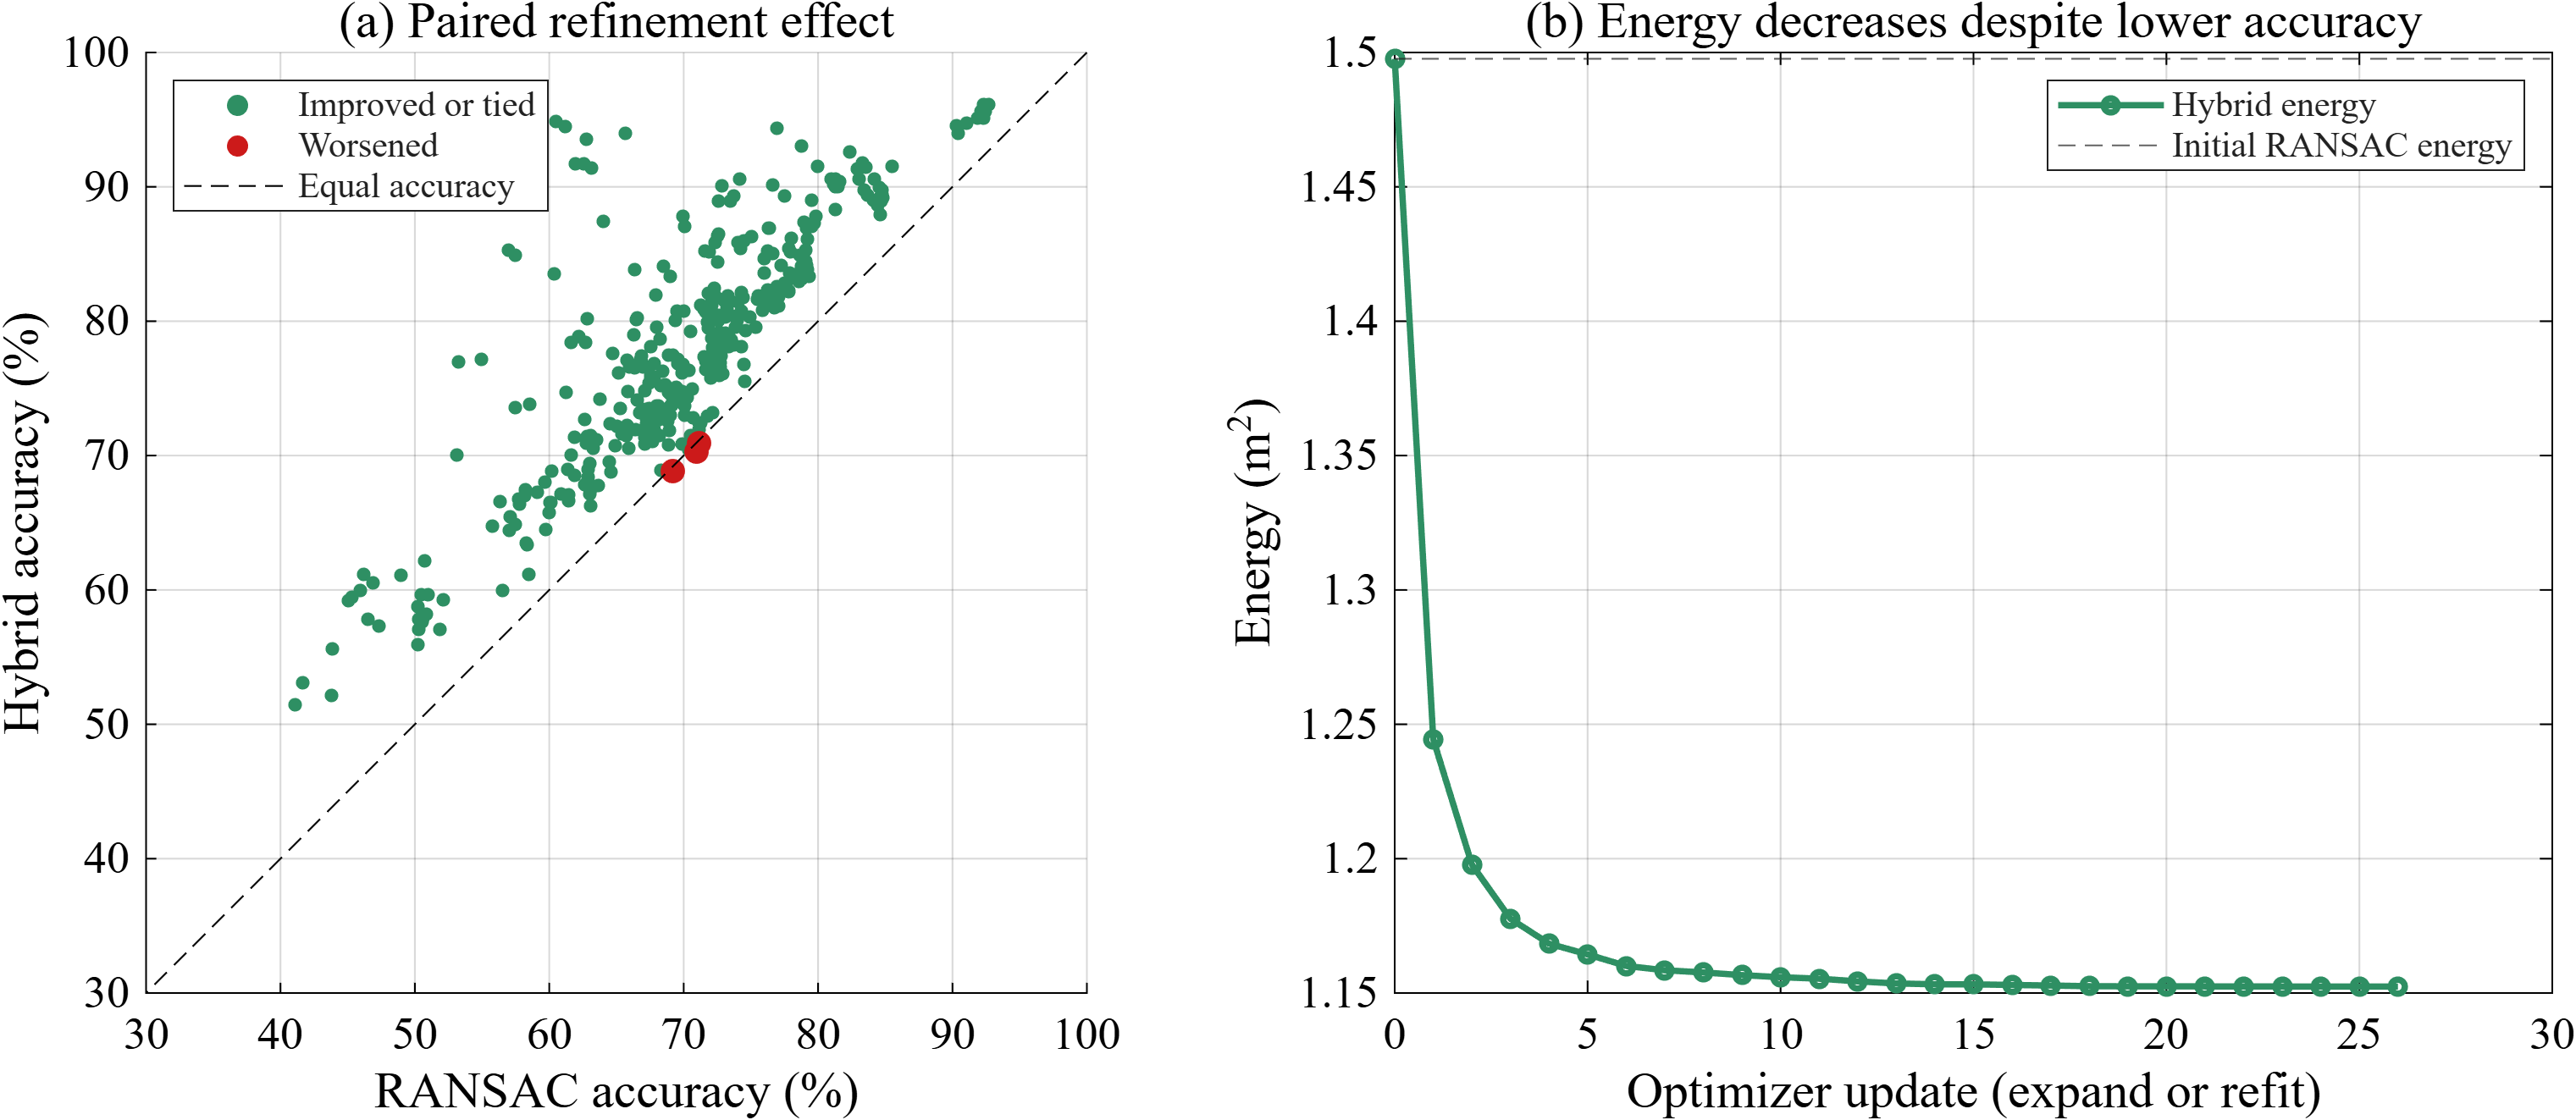
\includegraphics[width=\textwidth]{figures/results_paired_energy.png}
\caption{(a) Paired point accuracies for all 360 RANSAC and hybrid records; red markers identify the three decreases. (b) Hybrid energy history for test pc\_25, var1, seed 19, the largest accuracy regression. Energy decreases from 1.4977 to 1.1524 even though accuracy falls from 70.97\% to 70.26\%. Updates alternate expansion and refitting; the plot does not imply that intermediate accuracy was measured.}
\label{fig:results_paired_energy}
\end{figure*}

\subsection{Poorly segmented examples}\label{poorly-segmented-examples}

Fig.~\ref{fig:results_failure_cases} deliberately shows failure cases rather than visually favorable examples. The first is the scan--variant case with the lowest three-method mean point accuracy among seed-7 records. The second is the largest hybrid accuracy regression across all 360 paired records. These criteria make the selection reproducible, while the examples are not intended to estimate the prevalence of a failure pattern.

For test pc\_03, var4, seed 7, RANSAC achieves 41.63\% accuracy, sampled PEARL 64.52\%, and the hybrid 53.08\%. Matched IoUs are 0.1006, 0.2599, and 0.1518, respectively. The reference contains 57 planes, compared with 25, 77, and 25 extracted planes. The maps expose disagreement along boundaries and small supports. Sampled PEARL improves the segmentation but still leaves substantial plane-level errors; increased point accuracy should not be interpreted as complete structure recovery.

For test pc\_25, var1, seed 19, RANSAC accuracy falls from 70.97\% to 70.26\% after refinement, while matched IoU rises slightly from 0.0686 to 0.0716. Energy decreases by 0.3452. Thus, the optimizer improves its chosen objective and one overlap measure while worsening another evaluation measure. Both RANSAC and the hybrid return 17 planes for 69 reference planes. Sampled PEARL returns 92 planes and reaches 79.01\% accuracy, but its matched IoU remains only 0.2362. A good fit to large supports can coexist with many missed, merged, or fragmented smaller structures.

\begin{figure*}[!t]
\centering
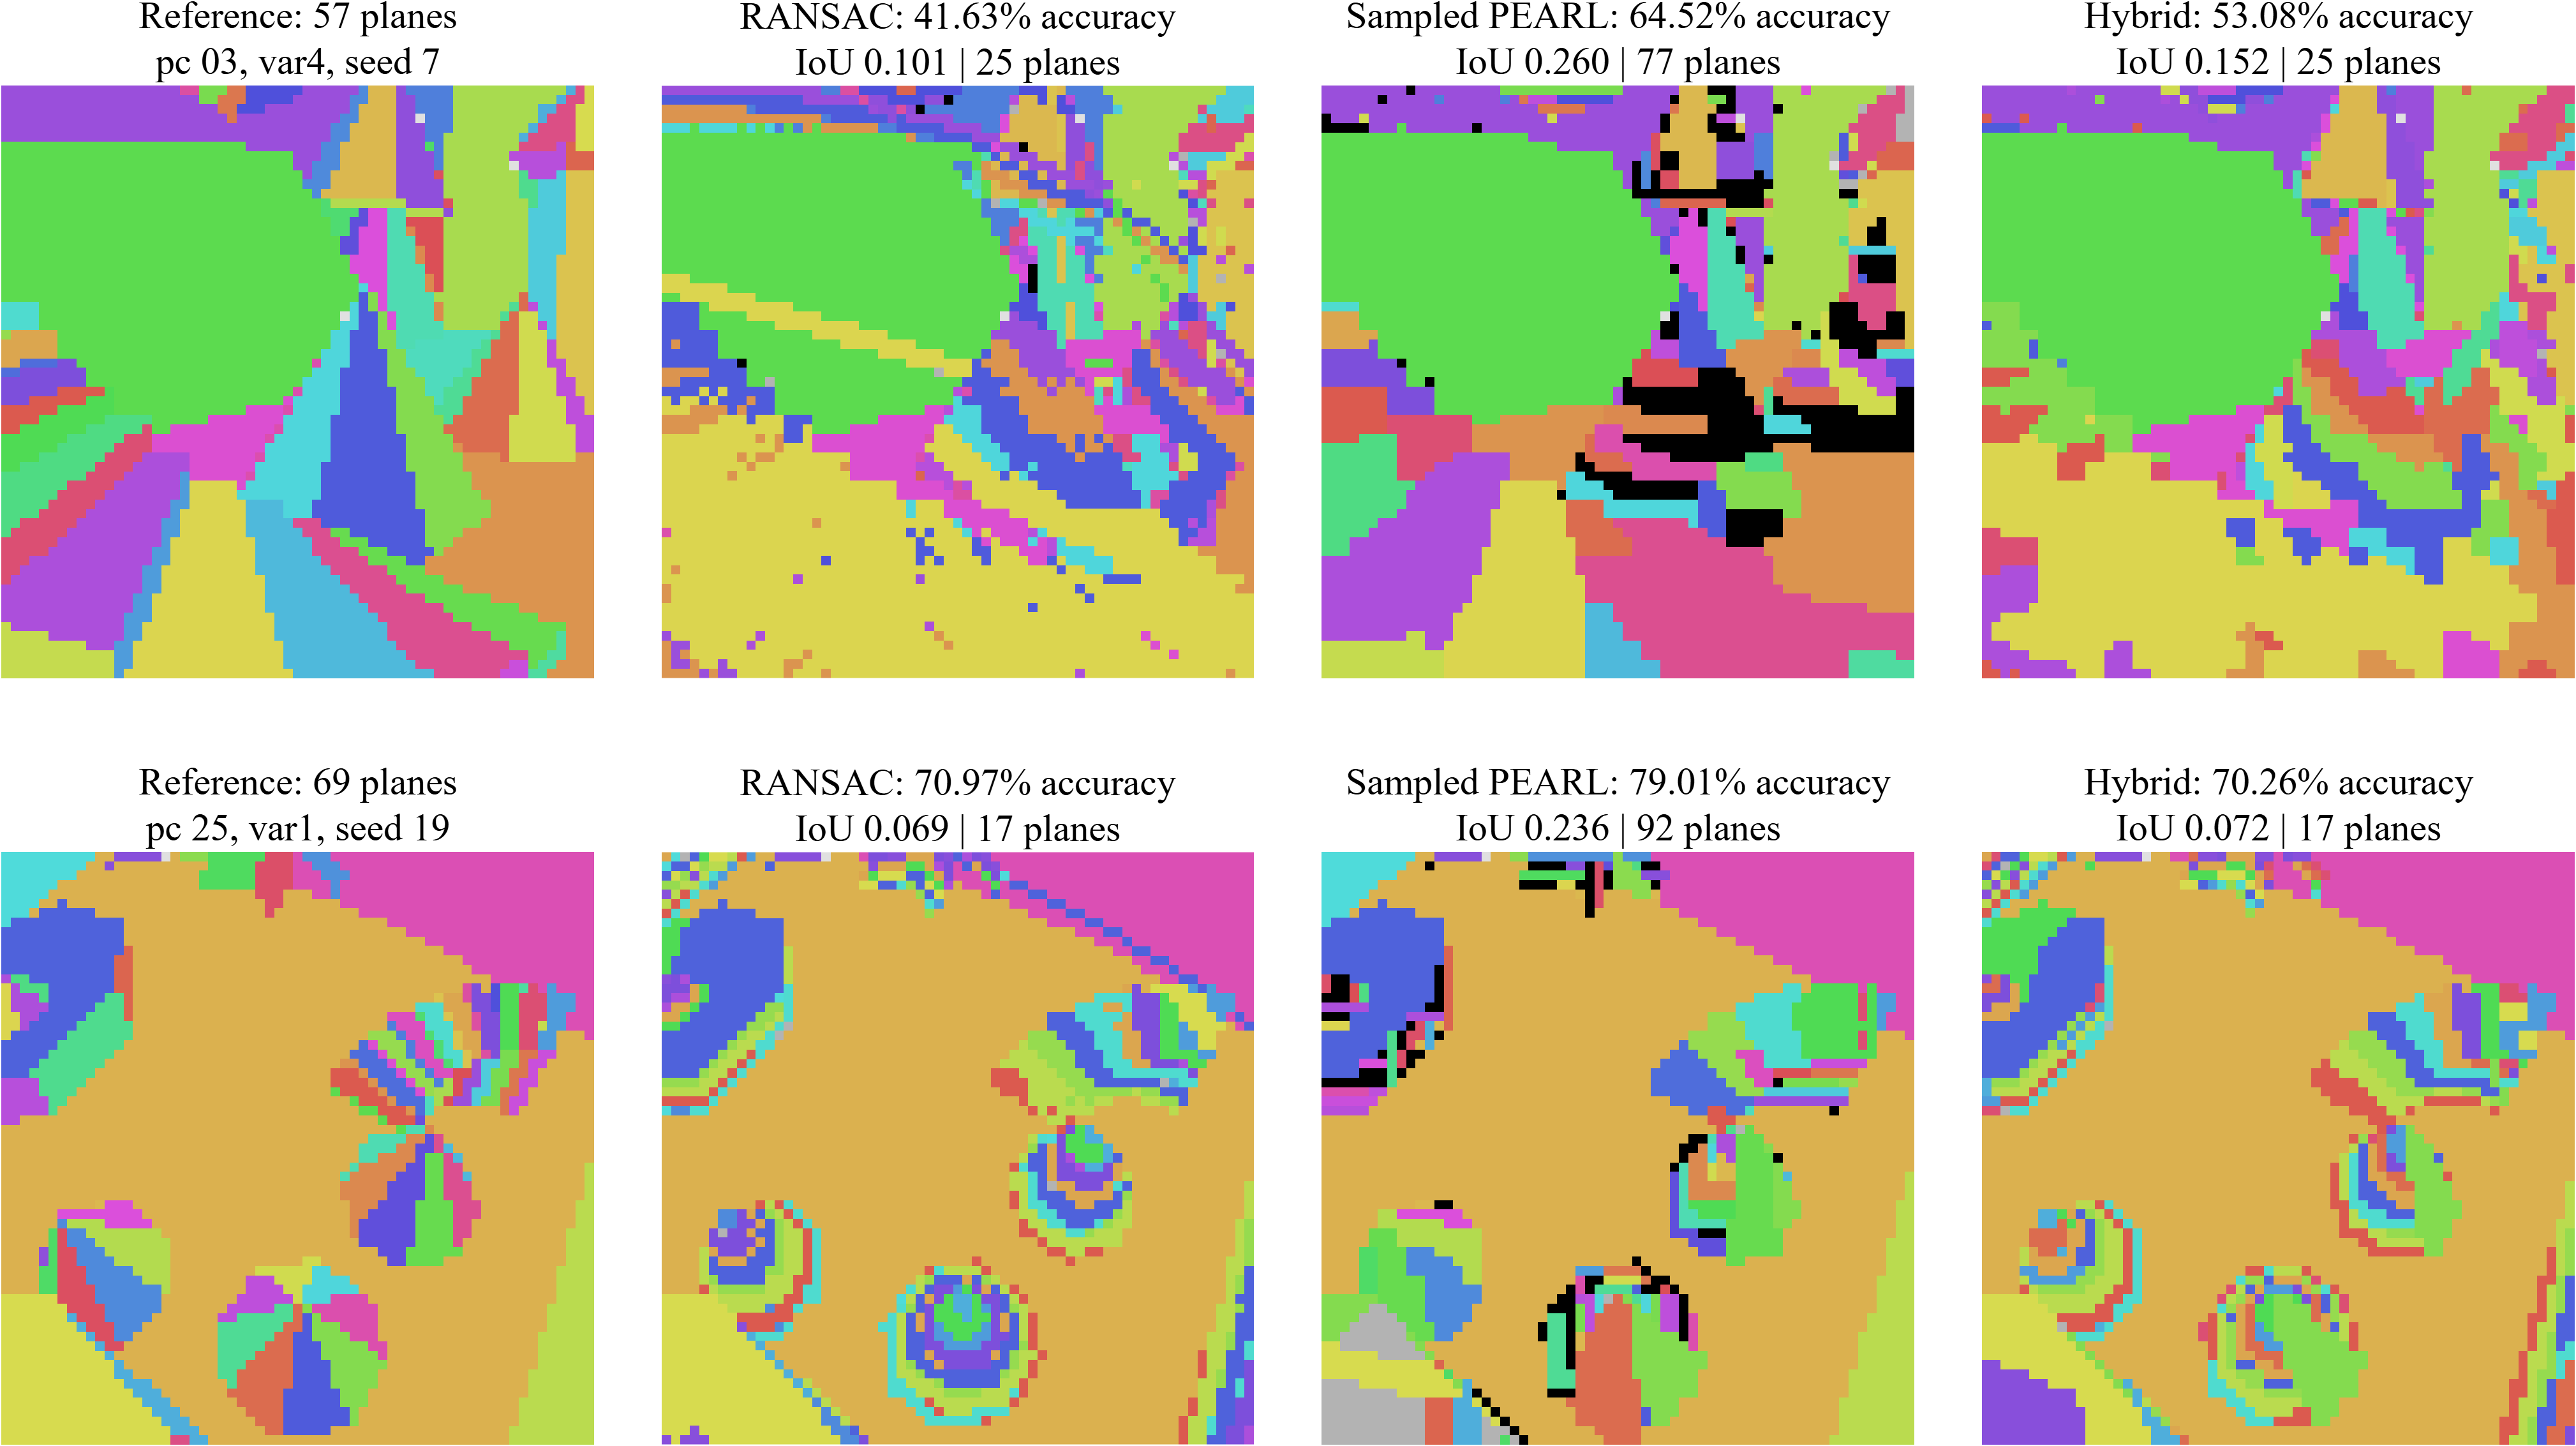
\includegraphics[width=\textwidth]{figures/results_failure_cases.png}
\caption{Saved predictions for the two explicitly selected difficult cases. Each row shows reference labels, RANSAC, sampled PEARL, and the hybrid on the organized stride-eight grid. Colors are aligned independently in each row by the same one-to-one matching used for evaluation. Black denotes an unmatched predicted plane, gray denotes rejection, and light gray denotes ignored reference points. A matched color identifies the mapped plane, not a guarantee that every point of that color is correct. Titles report point accuracy, mean matched IoU, and plane count.}
\label{fig:results_failure_cases}
\end{figure*}

\subsection{Spatial regularization ablation}\label{spatial-regularization-ablation}

The ablation compares sampled PEARL at \(\eta\) = 0.4 with the same pipeline at \(\eta\) = 0. Both conditions use the same input points, initial plane bank, data-cost scaling, and iteration budgets. Plane parameters are still re-estimated by SVD when the spatial term is removed. This is a test of spatial coupling under a fixed selected configuration, not a comparison with absent training or missing initialization. The generator is reset, but label-visit orders are not explicitly matched because the ablation skips proposal generation.

Table~\ref{tab:ablation} shows that mean accuracy falls from 84.26\% to 11.27\%, a decrease of 72.99 percentage points. Mean matched IoU falls from 0.4554 to 0.0746, and mean F-score from 0.4003 to 0.0005. The spatial-prior condition has greater accuracy and matched IoU in every paired record. Without the prior, all 150 candidate labels remain active in every case, compared with 54.25 active labels on average when regularization is present. The observed scattered assignments and retained label count are consistent with the lack of a penalty for spatial disagreement or model count in the unregularized objective.

\begin{table*}[!t]
\caption{Spatial-prior ablation over 360 records per condition. Runtime is measured within the separate ablation run and must not be mixed with the timing values in Table~\ref{tab:comparison}. Accuracy and overlap of the regularized condition reproduce the three-way comparison exactly.}
\label{tab:ablation}
\centering\footnotesize
\begin{tabular}{lrrrrr}
\hline
\shortstack{Condition} & \shortstack{Accuracy\\(\%)} & \shortstack{Matched\\IoU} & \shortstack{F-score} & \shortstack{Final\\planes} & \shortstack{Time\\(s)} \\ \hline
\(\eta\) = 0.4 & 84.26 \(\pm\) 8.31 & 0.4554 & 0.4003 & 54.25 & 36.497 \\
\(\eta\) = 0 & 11.27 \(\pm\) 3.76 & 0.0746 & 0.0005 & 150.00 & 27.526 \\
\hline
\end{tabular}
\end{table*}

\begin{figure*}[!t]
\centering
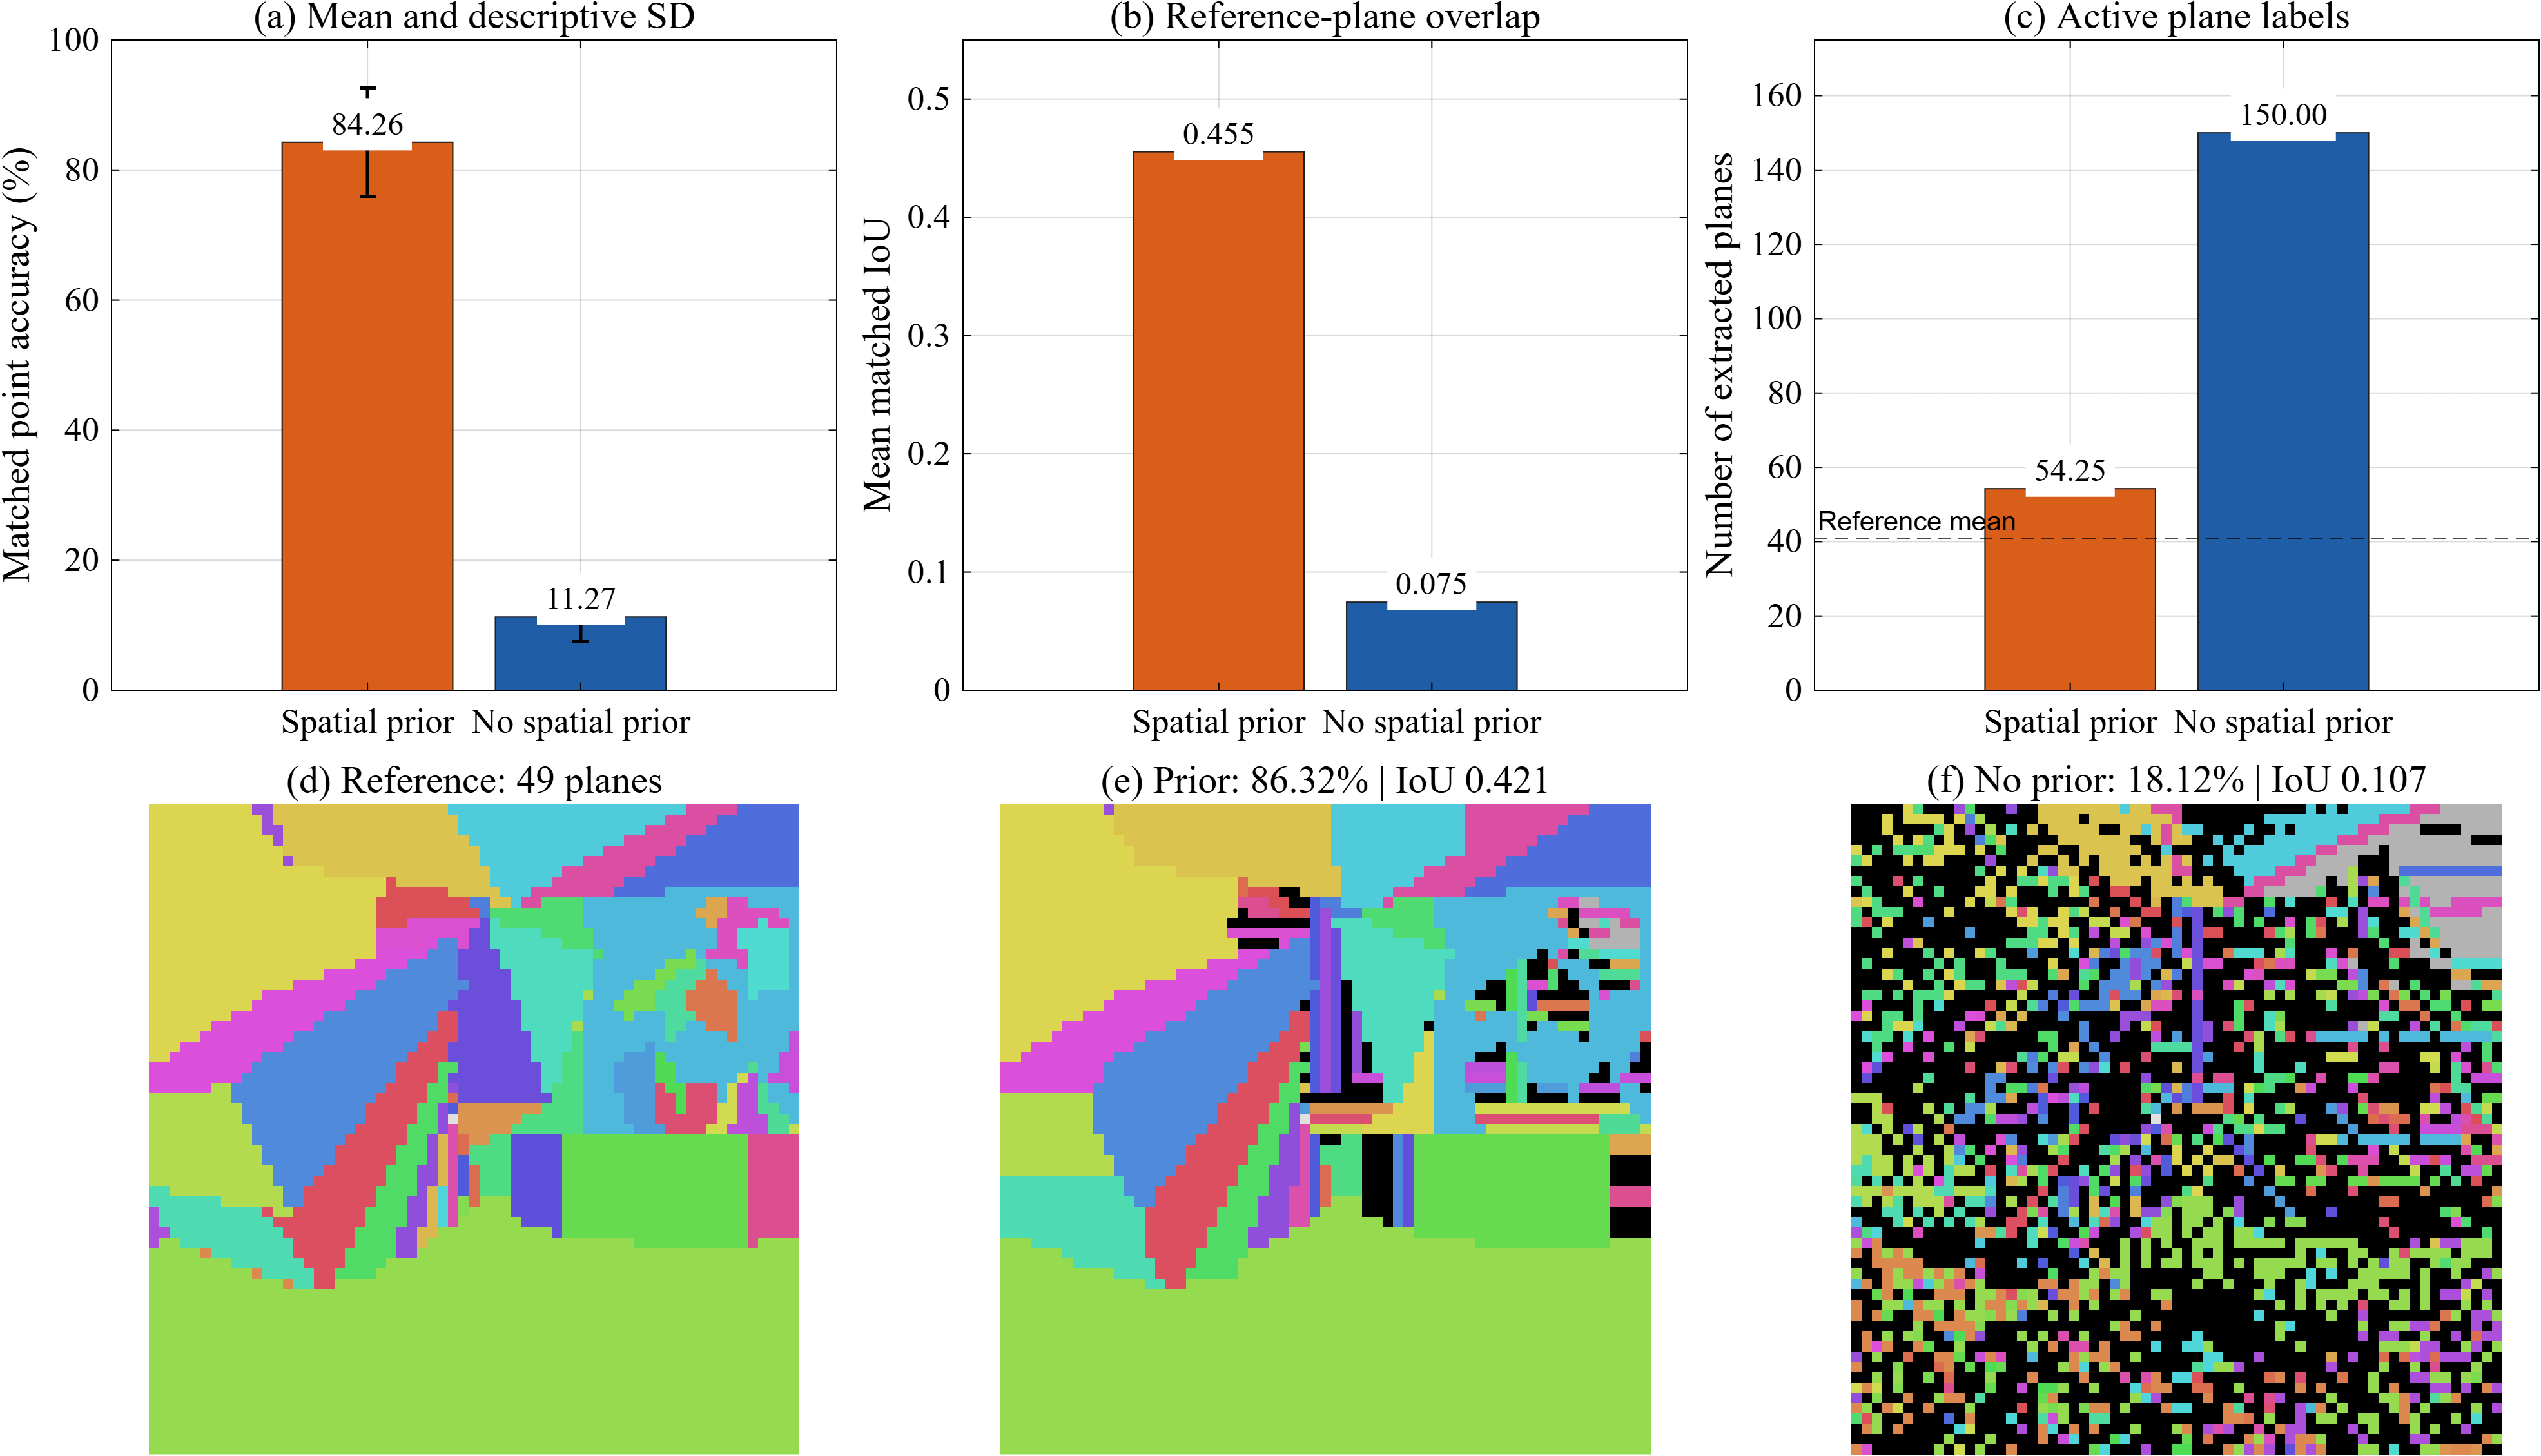
\includegraphics[width=\textwidth]{figures/results_spatial_ablation.png}
\caption{Aggregate ablation results and test pc\_12, var1, seed 7, selected at the lower median regularized accuracy among seed-7 cases. Both conditions use identical saved initial planes. The reference has 49 planes, compared with 74 with the prior and 150 without it. Colors follow Fig.~\ref{fig:results_failure_cases}. The unregularized result shows scattered, incorrect assignments despite SVD refitting.}
\label{fig:results_spatial_ablation}
\end{figure*}

The ablation run records mean times of 36.497 s with the prior and 27.526 s without it. Removing regularization therefore reduces runtime in that run, but the loss of segmentation quality is substantial. Although segmentation scores match the three-way run, its timings differ across sessions; the logs do not establish why. This study makes within-run timing comparisons and does not pool those runtimes.

\subsection{Interpretation and limitations}\label{interpretation-and-limitations}

Under the fixed protocol, refinement usually improves RANSAC, sampled PEARL gives better segmentation at greater cost, and spatial regularization benefits the selected configuration. The initialization experiment changes both models and labels, so it cannot isolate either factor. The \(\eta\) = 0 condition was not separately retuned; tuning it and matching label-visit orders would test the ablation's generality. Correlated records from synthetic scans do not establish significance from 360 independent scenes or real-world robustness. The failures show why point accuracy, overlap, model count, and energy must be interpreted together.
